\documentclass[a4paper]{article}
\usepackage[utf8]{inputenc}
\usepackage{graphicx}
\usepackage{tabto}

\title{Zusammenfassung Datenbanken}
\author{Heosibel}

\begin{document}

\maketitle


\begin{center}
    Sommersemester 2021 \\
    Professor: Dr.-Ing. Maik Thiele
\end{center}

\,

\begin{center}
    Dieses Dokument enthält eine Zusammenfassung der Vorlesung Datenbanken vom SS 2021.
    Diese Dokument ist kein offizielles vom Lehrstuhl und sollte nicht als Referenz verwendet werden.
    Die Erstellung ist in Vorbereitung auf die Prüfung im SS 2021 aus den Folien geschehen und kann Ungenauigkeit und/oder Fehler enthalten!
\end{center}


\newpage

\section{Einführung}

\subsection{Definition Datenbank}
\begin{itemize}
    \item logisch konsistent  
    \item besitzt eine bestimmte Bedeutung
    \item repräsentiert einen Ausschnitt der realen Welt
\end{itemize}

\subsection{Ziel einer Datenbank}
\begin{itemize}
    \item effektives + effizientes Speichern
    \item Wiederfinden von Daten
    \item Analyse von Daten
\end{itemize}

\subsection{Gründe für DBS}
\begin{itemize}
    \item Effizienz und Skalierbarkeit
    \item Fehlerbehandlung und Toleranz
    \item Mehrbenutzersynchronisation
    \item Sicherstellung der Datenintegrität
    \item Deklarative Anfragesprachen ( Benutzer sagt was und nicht wie die Daten geholt werden)
    \item Datenunabhängigkeit
\end{itemize}

\subsection{ANSI-SPARC-Architektur}
\begin{itemize}
    \item Externe: Definition externer Schemata (Nutzer oder anwendungsspezifische Sichten)
    \item Logische: definiert die logischen Datenstrukturen und deren Beziehungen
    \item Interne: Festlegung der Art und Weise der Speicherung
\end{itemize}

\begin{figure}[htp]
    \centering
    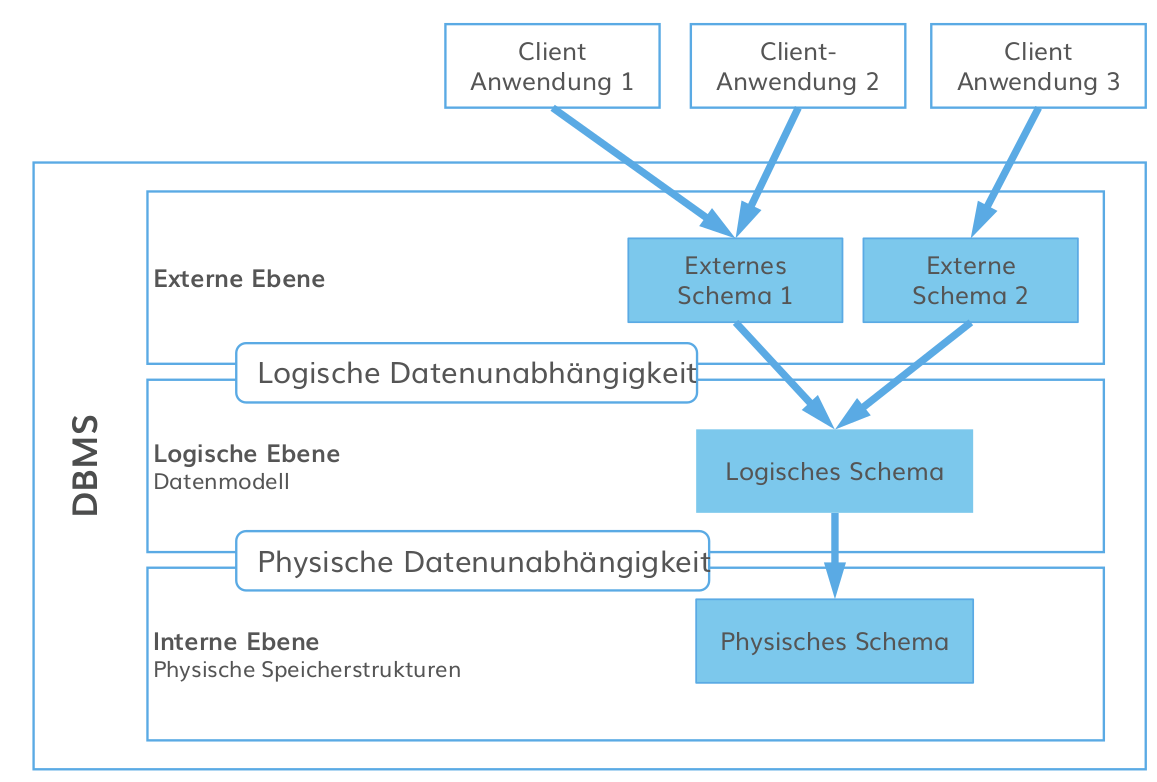
\includegraphics[width=9cm]{images/ANSI-SPARC}
    \caption{ANSI-SPARC-Architektur}
    \label{fig:ANSI-SPARC}
\end{figure}

\subsection{konzeptuelle Modelle}
\begin{itemize}
    \item Entity-Ralationship-Modell (ER-Modell)
    \item Unified Modeling Language (UML)
\end{itemize}

\subsection{Logische Modelle}
\begin{itemize}
    \item Hierarchische Modelle
    \item objektorientierte Modell
    \item Netzwerkmodelle
    \item Relationale Modelle
    \item ...
\end{itemize}

\subsection{Datenverwaltung ohne DBMS (Probleme)}
\begin{itemize}
    \item kein standardisiertes Format
    \item Duplikate
    \item hoher Aufwand bei Kombination von Daten
    \item Dateninkonsistenz
    \item maßgeschneidert aber ineffizient
    \item kein Mehrbenutzerzugriff
\end{itemize}

\newpage

\subsection{Information Retrieval}
\begin{itemize}
    \item Def: finden von Information unstrukturierter Art das eine Informationsnachfrage genügt
    \item Aufgabe:
    \begin{itemize}
        \item Suche nach Informationen
        \item Strukturierung von meist unstrukturierten Daten
        \item Befriedigung des Informationsbedürfnisses eines Benutzers
        \item Bewältigung von großen Datenmengen
    \end{itemize}
\end{itemize}

\subsection{Arten von Daten}
\begin{itemize}
    \item strukturierte Daten (z.B. Relationen)
    \item unstrukturiert Daten 
    \item semistrukturierte Daten
\end{itemize}

\newpage

\section{Konzeptueller Entwurf}

\subsection{Phasen des Entwurfes}
\subsubsection{Konzeptueller Entwurf}
\begin{itemize}
    \item semantisches Modell der Objekttypen
    \item Beziehungen der Objekttypen
\end{itemize}

\subsubsection{Logischer Entwurf}
\begin{itemize}
    \item Transformation semantischen Modells in DBS-spezifisches Datenmodell
    \item z.B. ER-Modell
\end{itemize}

\subsubsection{Physischer Entwurf}
\begin{itemize}
    \item Einrichten der Datenbank + internes Schemata
    \item eventuell laden von Daten
\end{itemize}

\subsection{Entity-Relationship-Modell}
\begin{itemize}
    \item Entität: existiert in der Welt und unterscheidet sich von anderen Entitäten
    \item Attribut: relevantes Merkmal
    \item Beziehung: Zusammenhänge zwischen Entitäten
\end{itemize}


\subsection{Funktionalitäten}
\begin{itemize}
    \item One-To-One: (1:1) Beziehung von einer Entität zu höchstens einer anderen  
    \item Many-To-One: (1:N) 
    \item Many-To-Many: (N:M) Es liegt keine Beschränkung vor
    \item n-stellige Beziehungen (z.B. betreuen: Professoren x Studenten → Seminarthemen)
\end{itemize}

\subsection{Min/Max Notation}
\begin{itemize}
    \item min: jede Entität dieses Typs steht mind. min-mal in Beziehung
    \item max: jede Entität dieses Typs steht höchstens max-mal in Beziehung
    \item Sonderfälle
    \begin{itemize}
        \item min = 0: braucht keine Beziehungen
        \item max = *: kann beliebig oft in Beziehung stehen
    \end{itemize}
\end{itemize}

\begin{figure}[htp]
    \centering
    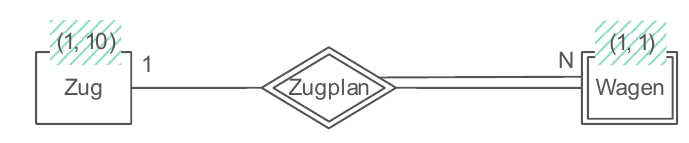
\includegraphics[width=9cm]{images/MinMaxNotation.png}
    \caption{Min-Max-Notation Beispiel Zug}
    \label{fig:MinMaxNotation}
\end{figure}

\subsection{erweiterte Attribut-Typen}
\begin{itemize}
    \item zusammengesetzte Datentypen
    \item mehrwertige Datentypen
    \item abgeleitet Attributwerte
\end{itemize}

\subsection{Spezialisierung und Generalisierung}
\begin{itemize}
    \item jede Instanz der Subklasse ist auch Instanz der Klasse
\end{itemize}
\begin{tabular}{l p{10cm}}
    Generalisierung (bottom-up): &  Unterdrückung der Unterschiede der Objekte \\
    & \\
    Spezialisierung (top-down): & Betonung der Unterschiede \\
    & \\
    d (disjunkt): & Instanzen der Unterklasse disjunkt \\
    & \\
    o (overlap): & Instanzen können sich überlappen \\
    & \\
    totale Spezialisierung: & Jede Instanz der Superklasse muss mind. eine Instanz der Subklasse sein \\
    & \\
    partielle Spezialisierung: & eine Instanz kann zu einer Subklasse gehören \\
    & \\
\end{tabular}

\begin{figure}[htp]
    \centering
    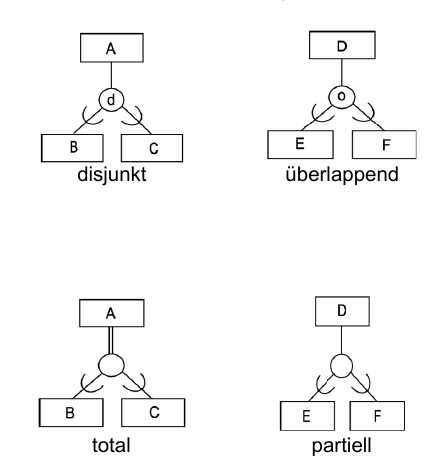
\includegraphics[width=6cm]{images/SpezialisierungGeneralisierung.png}
    \caption{Spezialisierung und Generalisierung Symbole}
    \label{fig:SpezialisierungGeneralisierung}
\end{figure}

\newpage

\section{Logischer Entwurf}

\subsection{Grundlagen}
\begin{tabular}{l p{10cm}}
    Tupel: &  Element einer Relation \\
    & \\
    Kardinalität: & Kardinalität einer Relation: Anzahl der Tupel in einer Relation \\
    & \\
    Relation & Menge von Tupeln \\
\end{tabular}

\subsection{Primärschlüssel}
\begin{tabular}{l p{10cm}}
    Eindeutigkeit: &  jeder Schlüsselwert ist einzigartig und nicht doppelt vertreten \\
    & \\
    Definiertheit: & Jedes Objekt hat einen Schlüsselwert \\
    & \\
    Minimalität & es kann kein Teil des Schlüssels weggelassen werden sodass immer noch die Eigenschaften \\
\end{tabular}

\subsection{Fremdschlüssel}
\begin{tabular}{l p{10cm}}
    Verwendung: &  Ausdrücken von Beziehungen (verweist auf eine andere Relation wo dieser ein Primärschlüssel ist) \\
    & \\
    Eigenschaften: & Definiertheit und Minimalität
\end{tabular}

\subsection{ER-Modell in Relationales Modell}
\begin{enumerate}
    \item Übersetzung von Entitäten
    \item Übersetzung von Attributen
    \item Übersetzung von 1:1 Beziehungen
    \item Übersetzung von 1:N Beziehungen
    \item Übersetzung von M:N Beziehungen
    \item Übersetzung von Beziehungen zwischen mehr als zwei Relationen
    \item Übersetzung rekursiver Beziehungen
    \item Übersetzung von Attributen an Beziehungen
    \item Übersetzung von Vererbungsbeziehungen
\end{enumerate}

\subsection{Abbildungsvarianten}
\subsubsection{Horizontale Partitionierung}
\begin{itemize}
    \item jedes Objekt ist genau ein Tupel einer Relation → gleiche ID heißt nicht das selbe Objekt
    \item Zusammenführung der Gesamtrelation entstehen viele NULL Objekte
\end{itemize}

\subsubsection{Vertikale Zerlegung}
\begin{itemize}
    \item Gesamtheit aller Attribute einer Objektes nur durch den Verbund erhaltbar
\end{itemize}

\begin{figure}[htp]
    \centering
    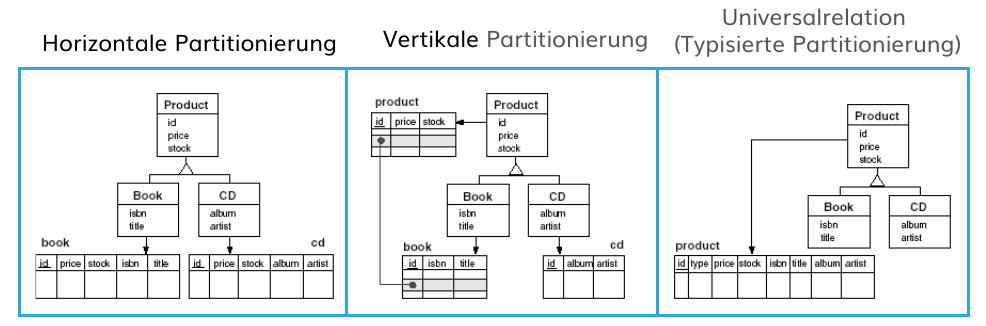
\includegraphics[width=14cm]{images/Partitionierung.png}
    \caption{Vertikale und Horizontale Partitionierung}
    \label{fig:Partitionierung}
\end{figure}

\newpage

\section{Relationale Algebra}

\end{document}
